\documentclass[12pt]{article}
\usepackage{times}
\usepackage{rotating}
\usepackage{setspace}
\doublespacing
\usepackage[letterpaper]{geometry}
\geometry{top=1.0in, bottom=1.0in, left=1.0in, right=1.0in}
\usepackage{dirtytalk}
\usepackage{csquotes}
\setlength\headsep{0.333in}
\usepackage{graphicx}
\usepackage{subcaption}
\usepackage{fancyhdr}
\pagestyle{fancy}
\lhead{}
\chead{}
\rhead{Gupta \thepage}
\lfoot{}
\cfoot{}
\rfoot{}
\renewcommand{\headrulewidth}{0pt}
\renewcommand{\footrulewidth}{0pt}

\newcommand{\bibent}{\noindent \hangindent 40pt}
\newenvironment{workscited}{\newpage \begin{center} Works Cited \end{center}}{\newpage }

\newenvironment{coverletter}{\begin{center} Cover Letter \end{center}}{\newpage }
\DeclareTextFontCommand{\booktitle}{\em}


\begin{document}
\begin{flushleft}


\begin{spacing}{2.0}
Harshita Gupta

Humanities Colloqium

April 26, 2017

\begin{coverletter}
\singlespacing

My conversation with Professor Miller helped to identify some key concerns with the experiments I was engaging in and why this was causing difficulty in interpretation. As he put it, I had ``too many degrees'' to my experiments, and was applying the meta-processes of close reading to experimental, almost scientific exploration, which needed, as he said, ''more controls``. I reduced the translations I was dealing with, reduced the role of the graphs and visuals in my interpretation, and focused on using preexisting analyses as my axes upon which to make interpretive moves or pivots via computational methods. 

When I cleaned the models according to the interests I expressed in draft, removing some rogue proper nouns and publishers notes, many of the trends that I'd identified in my draft, like the difference in occurrences of women, were no longer present. Generating the models with the parts of speech that I detected earlier, and with the topic number setting set to 15, also yielded cleaner, more meaningful topics that didn't have as many unreadable words or errors. Additionally, instead of simply using the top ten words in a topic, I used a threshold value to determine whether the topics coherence was statistically significant (threshold signal value); I felt like this was a representation that relied on a more rigorous understanding of the model's output.\linebreak

Perhaps the biggest 'lesson' I learned in this project is what Professor Miller said to me in our last conversation- ``I've made tons of cool shit that I have no idea what to do with, and will probably never know what to do with, because it doesn't provide much useful information''. My original revision was a very ambitious attempt at using networks to depict the thematic structures of the translations; I spent hours generating beautiful and intriguing network diagrams that while interesting creative projects, weren't taking me as far interpretively as more rigorous and 'simple' interactions with the model itself. I learned to let go of days of work to get to a more valuable product. I would be interested in discussing these with you in a more informal setting to see what you make of them!\linebreak

I think much of the difficulty with this paper was that I'm not as well trained in reading and interpreting models as I am in close-reading --- setting out on this project was a challenge in both, the model-creation respect, as well as in learning to productively and accurately interpret topic signals and force-directed network graphs.  If I'd had better training in this skill, I think I'd have had a much better return on investment with my time, and would've had better intuition for what experiments would be successful or not. \linebreak

Given more time and resources, I would certainly give these models and their results a more thorough treatment, with perhaps a more ``mesoanalytic'' lens --- since I wasn't able to read all four translations in depth, and was only interacting with models, the traditionalist in me (however small a part that may be) finds the result only partly satisfying. I would want to endeavor to correlate my network's results with clearer plot and thematic trends across the text, versus ones in specific scenes that the topics can point out; this would only be doable once I've read the entirety of each text.

\end{coverletter}


\begin{center}
Computationally Identified Domestication v. Foreignization of \booktitle{Genji} through ``Sad Love''
\end{center}

\setlength{\parindent}{0.5in}

In Metonymy in The Tale of Genji: An Analysis of Translation Strategies, Janel R. Goodman Murakami compares occurrences of metonymy in a passage across translations of the \booktitle{Tale of Genji} to assess how domesticated or foreignized Suematsu's, Waley's, Seidensticker's, and Tyler's translations are, concluding that the more modern translators retain foreign elements of the text more faithfully than their earlier counterparts. In ``Going to Bed with Waley: How Murasaki Shikibu does and does not become world literature,'' Valerie Henitiuk uses a similar microanalytic approach, more commonly referred to as close-reading, to analyze the scene of Genji's and Murasaki's consummation. She argues that while Seidensticker's  portrayal of the scene as rape and an act of aggression may initially appear feminist and progressive, it loses the opportunity to employ the ``far more subtle and thus profound criticism... to explore the insidious social problems at the very root of situations like this'' (Henitiuk 56). Seidensticker's portrayal, as well as Tyler's (though to a lesser extent), emphasizes the difficulties of the specific situation over the system at large, missing the larger social commentary that Murasaki Shikibu is making, or the ``true critique being leveled at prevailing attitudes and behaviors''. A successful critique, would be ``implicit but no less scathing'' (Henitiuk 57).

Henitiuk's conclusions are drawn based on close readings of a select few passages from each translation, a very microscopic approach for a text as varied and large in scope as \booktitle{Genji}. Her argument is based on the understanding that Seidensticker and Tyler misstep by setting apart this scene from the rest of the novel; Henitiuk is thereby relying on a fundamentally macroanalytic understanding of each translation's baseline for representing interactions amongst characters. This is where the definitively macroanalytic approach offered by computational analysis is useful. My paper draws out and tests the underlying assumptions to Henitiuk's microanalysis by offering a holistic, modeled understanding of each translation's thematic world to shed light on the portrayal of the morning-after scene in juxtaposition to the text as a whole. I ultimately discover that it is not simply a misinterpretation of Murasaki Shikibu's critique that weakens Seidensticker's rendition of the morning-after scene, but a larger failure to step outside his own cultural experience of love and relationships, specifically, in resolving negative emotion and relationships, that leads to his misreading of the text -- and while Tyler improves on this, it is Washburn's translation, that, despite possessing many of the problematic traits of Seidensticker's, maintains its foreign thematic structures of emotion, delivering the scene with the social commentary it was intended to provide.

In my endeavor to, like Murakami, evaluate the thematic and linguistic domestication versus foreignization of a translation, I turn to a work referenced by Henitiuk in ``Going to Bed With Waley,'' Margaret H Childs' ``The Value of Vulnerability: Sexual Coercion and the Nature of Love in Japanese Court.'' Childs analyzes the ``cross-cultural emotional experience'' and highlights the difference between modern American expectations of love and premodern Japanese literary representations of it. Her preliminary statements are about general categories of emotion, drawing attention to studies that show that the American schemas of emotion differ from Chinese ones in their inclusion of surprise, while Chinese ones differ from the American in their inclusion of shame, but the crux of her discussion is around the un-American category of loving feelings called 'sad love' depicted in Japanese literature, a category associated with negative emotions and words like 'pity' and 'pathetic'. There is a high correlation between fragility and beauty, and vulnerability and attraction.

Using Childs' research to set up these measurable variables to determine the ``westernization'' of a text --- through its cooccurring depiction of love and negative emotion --- sets the stage for technical models to take over and offer information about where each text falls on the spectrum of domestic to foreign. The appropriate tool for an analysis of negative emotion is sentiment analysis, a natural language processing tool that determines the positive or negative polarity of a word. I conducted sentiment analyses on the three translations in concern and displayed a histogram of the results for each text. \footnote{All sentiment scores with an absolute value of less than 0.0001 were excluded from the graphs, since they provide little interpretive value.}

\begin{figure}
	\begin{subfigure}{.3\linewidth}
		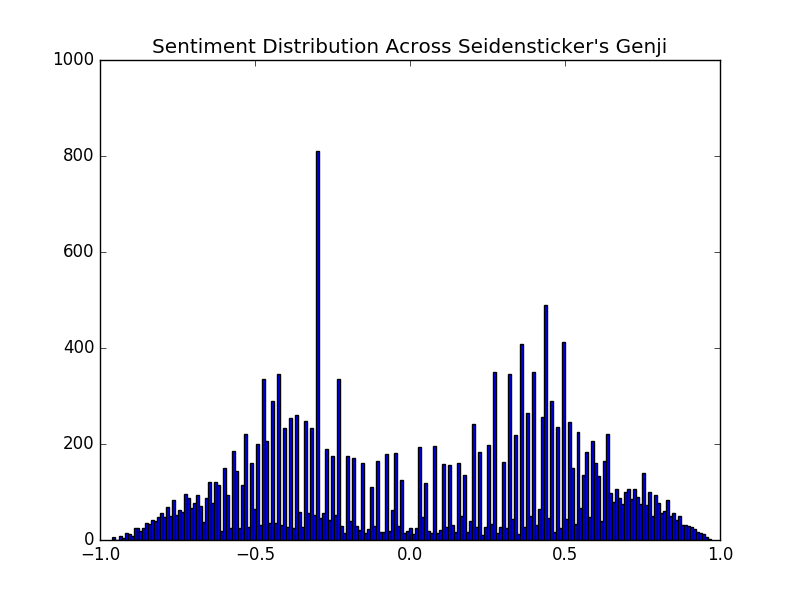
\includegraphics[width=2in]{seidensticker-sentiment.png}\hfill
		\caption{\scriptsize Median: 0.23, Mean: 0.04, Variance: 0.1772}
	\end{subfigure}
	\begin{subfigure}{.3\linewidth}
		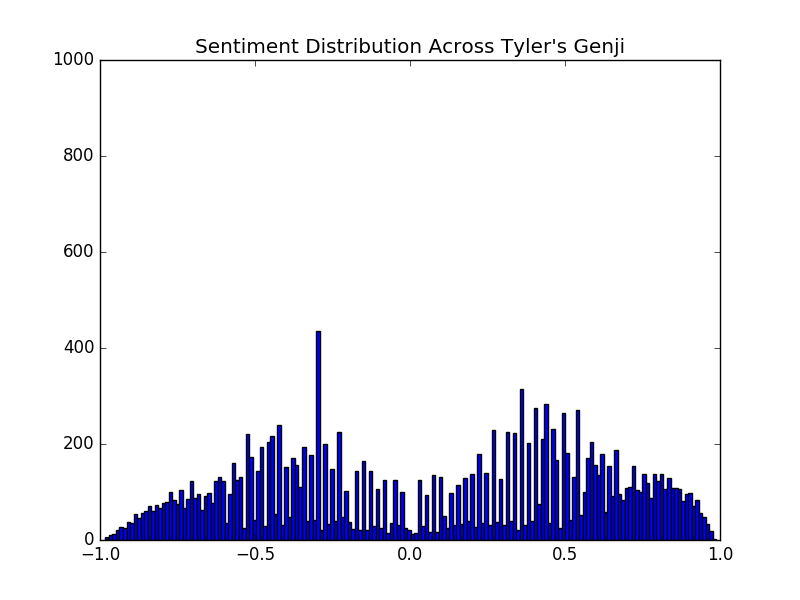
\includegraphics[width=2in]{tyler-sentiment.png}\hfill
		\caption{\scriptsize Median: 0.28, Mean: 0.06, Variance: 0.067}		
	\end{subfigure}
	\begin{subfigure}{.3\linewidth}
		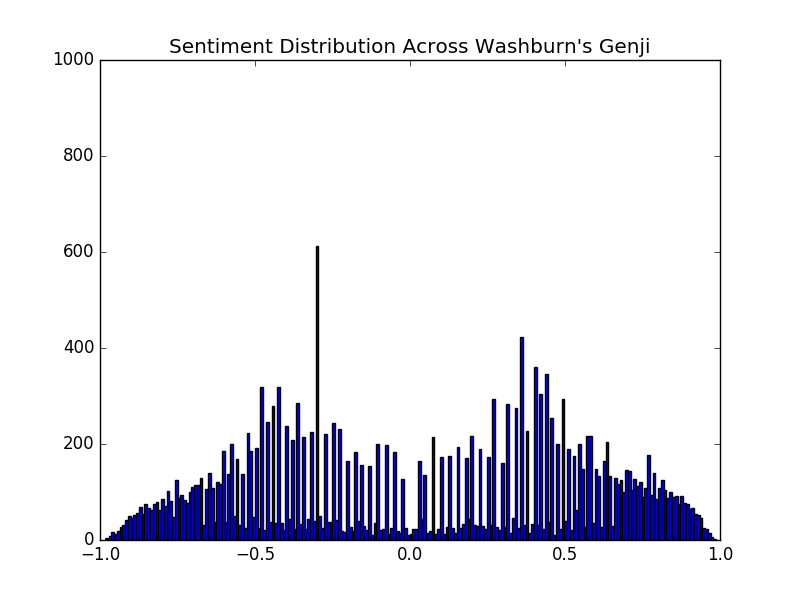
\includegraphics[width=2in]{washburn-sentiment.png}
		\caption{\scriptsize Median: 0.28, Mean: 0.04, Variance: 0.0772}
	\end{subfigure}
    \caption{Positive and Negative Sentiment Across \booktitle{Genji}}
    \label{sentiment-hists}
\end{figure}

An analysis of the histograms, along with the mean, median, and variance of the data, shows that Seidensticker's text is markedly more variant in its depiction of emotion, with a heavier clustering of values towards the edges of the graph than the other two texts. All the graphs have a much smaller mean than a median, which shows that the mean is skewed by some very low sentiment scores --- this is no surprise, as any reader of \booktitle{Genji} can surmise that the book is rife with dramatic, often heart-wrenching emotion. The presence of negative emotion in a plot filled with romantic entanglements suggests that the texts, and Seidensticker's most of all, are reasonably close to Childs' understanding of Eastern-language texts' depictions of love. Henitiuk's argument that Seidensticker's portrayal of the morning-after scene is anachronistic in its categorization of Genji as a rapist uses the extreme and sentimental language as its primary evidence. Therefore, is her argument challenged by the fact that Seidensticker's translation scores lower on sentiment across the text than Tyler's translation? If we use Childs' measures in this manner, then does this reveal that  Seidensticker is, in fact, truer to the original text? Since Seidensticker's language across the novel skews more negative than Tyler's, or in other words, he has a different emotional intensity baseline, Henitiuk's statement that he is westernizing the text with his usage of sentimentally intense words like ``shock'' and ``unscrupulous'' is reversed. This is, in fact, simply a function of Seidensticker's more sentimental translation as a whole, which is a function of his translation being the most true to the Japanese emotional world.

The caveat in this interpretation is that it is an oversimplified sentiment analysis, and reveals only the presence of negative emotion across the entirety of the text's plot, not its cooccurrence in romantic contexts. To determine whether there is meaningful cooccurrence between negative-sentiment-scoring words and love, or in other words, whether the translation is true to ``sad love,'' I turn to topic modeling. 

I apply digital topic modeling to break down and analyze the three translations of Genji in concern: Edward G. Seidensticker's from 1976, Royall Tyler's from 2001, and Dennis Washburn's from 2015 \footnote{ My greatest interest was originally in comparing the work of male translators with Helen McCullough's partial translation. Unfortunately, McCullough's translation, published only in \booktitle{Genji and Heike: selections from the Tale of Genji and the Tale of the Heike}, is heavily copyrighted and unavailable in any digital format.}. Topic modeling is a natural language processing technique that uses the principle of distributional semantics, or the common cooccurrence of two words, to group words into ``topics.'' I use the Latent Dirichlet Allocation (LDA) topic modeling method, which operates on 1000-word sequential chunks of the tale of Genji. LDA treats each ``chunk'' of words as an entity composed of ``topics'' --- each topic is composed of words that commonly occur together. A statistical explanation of LDA modeling's assumptions and mechanisms is beyond the scope of this paper, and one can turn to Rhody's ``Unpacking the Assumptions of LDA'' or Jockers' Macroanalysis for a simplified analysis of the method. Crucial to this paper and its discussion, however, is LDA modeling's unsupervised nature. Topics are not produced based on the program's understanding of the words' meanings or potential similarity, but creates buckets for topics based on the position of words relative to each other, and their common cooccurrence, i.e. distributional similarity, to determine that they belong to a similar topic. Its unsupervised nature makes LDA modeling useful for identifying topics in a more ``objective'' fashion by identifying authors' subconscious placement of words and themes and therefore reflecting their gendered and cultural inclinations. Topic modeling is useful, therefore, not just due to ability to give us a zoomed-out, abstracted view of a text as large as Genji, but also in uncovering topics that might be outside our microanalysis-based understanding of discoverable topics.

Topic modeling is traditionally applied to multiple documents that are dissimilar, as in the work by Jockers, and has been trained on corpuses containing multiple texts, 4500 poems in Rhody's case and 4500 texts in Jockers' case. These models develop generalized, often easily identifiable themes that can apply to texts across time and author, like Rhody's ``night light moon stars day dark'' and ``tree green summer flowers grass'' topics. Jockers' and Rhody's topics reveal nothing surprising in their content themselves; the combinations of words are predictable. Topic modeling of the form they practice is useful when the purpose of the topics, albeit predictable, is to be used later in topic distribution comparison across texts, but is less useful when working with a single text. I train the LDA model, instead, on a single translation of Genji at a time, thereby developing topics that are far more specific to each translation's ``thematic world,'' and useful in identifying the thematic differences underlying each translation. The interpretive advantage to this method is evident in the difference between the topics generated by the two cited authors, and the ones I display and analyze in my paper.

\begin{figure}
\caption{Topics in Seidensticker's Translation}
\label{seidensticker-topics}
\singlespacing
\small
Topic 1: stag softer curt outstandingli inwardli recast

Topic 2: seem come said t even see littl bishop dream came child look old girl 

Topic 3: seem robe paint red princess ladi women line littl white string master nose now 

Topic 4: girl ladi said seem thought think come now t look littl even know daughter good young time see women mother make came much go well man way princ 

Topic 5: seem thought even think come see now said go ladi princess time thing littl women make know world long want much day way say made feel look came still noth father 

Topic 6: emperor princ thought seem ladi court chines crown daughter present palac time son said year royal 

Topic 7: princ ladi emperor said blossom kobai daughter thought carriag even 

Topic 8: seem thought women littl governor even young room ladi look light said came back open away door wind way see day veranda 

Topic 9: emperor time now matter tear princ minist empress 

Topic 10: seem ladi safflow quarter white look 

Topic 11: ladi seem thought now time day even said year come see old princess came made much littl 

Topic 12: seem ladi thought daughter year come old think said son day thing well great made man 

Topic 13: t man thing good governor say seem girl think make look know go happen said woman daughter wife one want young day come even just don ve sort someon see everyth peopl m let ask 

Topic 14: emperor ladi court cat princ son crown mother third new father go see royal 
\end{figure}

\begin{figure}
\caption{Topics in Tyler's Translation}
\label{tyler-topics}
\singlespacing
\small
Topic 1: high paper great shoot book write cup scroll command son 

Topic 2: now high even look said way well still thought never time see littl go come long know feel seem day just thing ladi 

Topic 3: play captain old tale now flute music never ladi feel said seem life day hear say even 

Topic 4: majesti now flower light even wind long morn said dew day 

Topic 5: blossom look command made flower ladi littl spring beauti year 

Topic 6: now monk day world holi long mountain come adept wind littl captain thought citi know rever sent look way time 

Topic 7: rever nun young woman lordship go die come mother said even someon tell now noth high see look seem ask never sure just back told heard well happen talk sister women mistress 

Topic 8: majesti flower spring autumn ladi nun music year pine east quarter made consort wing long blossom high garden color 

Topic 9: captain young excel high play look lieuten son music blossom said right just seem man dress one even well make daughter come ladi secretari advis 

Topic 10: even now old play novic high noth often see biwa 

Topic 11: ladi gown look dress comb box one never mistress even high far day now cathay plum 

Topic 12: now long majesti littl thought day mani ladi made year see said well citi time still even come go look 
\end{figure}


\begin{figure}
\caption{Topics in Washburn's Translation}
\label{washburn-topics}
\singlespacing
\small
Topic 1: go ladi just woman feel come girl know even way said make think now nurs tell ask littl man lord night well look time dont attend see thought place 

Topic 2: carriag go feel wife process men view attend ladi just way blind space 

Topic 3: feel husband now even ladi emot heart deep woman say 

Topic 4: made lotu attend third minist flower make 

Topic 5: even capit boat day governor sea attend provinc ladi wind perform lord dream wave 

Topic 6: robe look ladi poem even day garden now seem blossom color tree made women 

Topic 7: cat third princess princ son crown littl blind robe felt see look close game face never contest think tri remark 

Topic 8: even feel now time world look thought see come ladi live heart felt just princess long villa day go 

Topic 9: father hardli wife 

Topic 10: time daughter son even emperor palac princ princess now father court look day year majesti third minist mani feel ladi world left 

Topic 11: play koto string instrument perform princess even music young son boy littl seem flute hear time daughter look major just robe women feel 

Topic 12: woman make way even man young just time now thing matter go mani 

Topic 13: princess even look feel young daughter woman man just ladi now go think women make time way captain letter thought see thing say come still 

Topic 14: ladi wind princess day ceremoni daughter father come carriag 
\end{figure}

Developing meaningful topics is not just a matter of corpus scale, but also of corpus content: following Jockers' guidance, I remove all stop words that do not provide interpretive value, like articles and pronouns, from the corpus before I discover themes within it. In ``Theme'', Jockers proposes and demonstrates topic modeling only on a corpus of common nouns. Restricting the corpus to nouns is appropriate in his use case as his corpus is much larger than a single \booktitle{Genji} translation, and therefore filtering for nouns allows for a higher level of abstraction that focuses on broader trends that are more likely to occur across hundreds of texts. In analyzing \booktitle{Genji}, however, restricting my models to only nouns results in a loss of rich nuance which is central to a cross-translation comparison: adjectives, adverbs, and verbs contain a wealth of information about emotion, description, and subjectivity. To this end, I include adverbs, adjectives, and verbs in my topic models.\footnote{ In addition to removing stop words and parts of speech other than the ones specified, I removed all annotations, introductions, publishers' notes, footnotes, and endnotes. In the Tyler translation, this included the deletion of all chapter titles that are not from the original, chapter introductions, and the ``Persons'' and ``Relationship to Previous Chapters'' sections. Additionally, all words are reduced to their stems - therefore treating ``respect'' and ``respectfully'' as identical semantic units and indistinguishable to the LDA algorithm. I also exclude all proper nouns from the corpus used for the topic model, so that topics are identified not upon the basis of scene (which correlates highly with proper nouns like names and places) but upon common motifs. Special care was taken to exclude all Japanese proper nouns, which are not identified by Western natural language processing tools.} The topics discovered, with the words that have the highest percentage of appearance within a given topic, are included in figures \ref{seidensticker-topics}, \ref{tyler-topics}, and \ref{washburn-topics} \footnote{All words in a given topic with signal strength greater than 0.0040 are included, i.e. words that comprise more than four percent of a given topic. If a topic had no words with signal strengths high enough, i.e. the topic was statistically insignificant, those topics were excluded from the final model and not used in subsequent discussion.}.

The topic model offers a probabilistically-sound way of determining association between concepts like pity and love: if they cooccur in a topic, they do so because the model has identified that they are distributionally similar and closely codependent within the thematic world of the corpus, in this case a single translation of Genji. To further study the existence of ``sad love'' across the translations, I generate a list of the ten most negative words in each translation, and then feed these words to the topic models and determine which topics each word is most likely to occur in --- more of the words occurring in topics about love or romance is taken as a quantitative indicator of depictions of ``sad love.'' My results are detailed in figures \ref{seidensticker-sentiment-topics}, \ref{tyler-sentiment-topics}, and \ref{washburn-sentiment-topics}. \footnote{Words that had no strong association with any topic were not included.} 

\begin{figure*}
	\caption{Seidensticker's Most Negative Words and the Topics They Belong to, Strongest Matches Listed First}
	\label{seidensticker-sentiment-topics}
	kill: 14, 2
	
	tragedy: 4
	
	evil: 5, 4
	
	devil: 2, 5
	
	murder: 14
	
	dead: 9, 7, 4, 5, 14, 6, 11, 2, 12
	
	devastating: 8
	
	hate: 5, 2, 8, 14, 11
	
	abuse: 8
	
	hatred: 9
	
	All themes correlated with negative sentiment words, most common listed first: 5, 14, 2, 8, 4, 9, 11, 7, 6, 12
\end{figure*}
\begin{figure*}
	\caption{Tyler's Most Negative Words and the Topics They Belong to, Strongest Matches Listed First}
	\label{tyler-sentiment-topics}
	hate: 2, 13, 9
	
	murder: 8
	
	kill: 8
	
	tragedy: 7
	
	evil: 8, 5, 2
	
	heartbroken: 8
	
	dead: 8, 4
	
	devastating: 5
	
	betray: 4, 5, 15, 7, 2, 14
	
	disast: 10, 2, 9
	
	All themes correlated with negative sentiment words, most common listed first: 8, 2, 5, 4, 7, 9, 10, 13, 15, 14
\end{figure*}

\begin{figure*}
	\caption{Washburn's Most Negative Words and the Topics They Belong to, Strongest Matches Listed First}
	\label{washburn-sentiment-topics}
	kill: 5
	
	hell: 3, 8, 14
	
	suicide: 1
	
	tragedy: 8
	
	evil: 3, 5, 8
	
	excruciating: 1
	
	dead: 8
	
	devastating: 8, 12
	
	hate: 12, 1, 9, 15, 14, 11, 8
	
	betray: 8, 10
	
	hatr: 5, 1
	
	crisis: 12
	
	All themes correlated with negative sentiment words, most common listed first: 8, 1, 5, 12, 3, 14, 10, 9, 15, 11
\end{figure*}

The more intricate experiment that topic modeling offers contradicts the simplistic view that sentiment analysis offered --- representations of ``sad love'' are least apparent in Seidensticker. In his translation, the correlation between negative words and romantic and love-focused themes is weak: the topics have stray mentions of women, but are much more court-focused (see topic 14 and 2) and ceremony-focused. In Tyler, there is a high correlation of nature and music with negative sentiment, but only one of the first five topics (topic 7) can be connected to love and romance, and only peripherally. In Washburn's translation, however, all of the first five negative-correlated themes are romantic or love-focused, with words like 'feel', 'heart', 'dream', 'emot', and 'deep.' Using this different measure of assessing Westernization reveals conclusions more in line with Murakami's, with Seidensticker's translation being more domesticated than Tyler's. Examining Washburn's thematic structure using Childs' measures in this way provides a methodology to place Washburn on Murakami's scale as well, deeming it the most foreignized of the translations examined. Washburn's translation's underlying linguistic associations reveal an investment in cultural subjectivity and translator invisibility at the cost of audience comprehensibility, therefore revealing goals of accurate portrayal rather than successful Western consumption. Washburn is, by far, the translation that maintains the text's unique contextual identity most faithfully. 

The determination, then, that Seidensticker's inaccurate portrayal is not in his exaggerated portrayal of negative emotion in the morning-after scene, but in his contextualization of negative emotion on a larger, text-wide scale, changes Henitiuk's conclusion. Seidensticker fails in his inability to grasp the realities of emotion in the world of \booktitle{Genji}, misplacing sentimentality as more related to societal and courtly functions like ceremony, and therefore to a world intricate yet removed from interior subjectivity. A translation like Washburn's, on the other hand, with a more faithful representation of the cultural and emotional thematic structure of \booktitle{Genji} and a conception of ``sad love'' preserved over the course of the text, delivers Murasaki Shikibu's ``implicit yet scathing'' commentary with grace.

\begin{workscited}

\bibent Jockers, M. L..\booktitle{Macroanalysis: Digital Methods and Literary History}. Champaign: University of Illinois Press, 2013. Project MUSE.

\bibent Rhody, Lisa M. ``Topic Modeling and Figurative Language.'' \booktitle{Journal of Digital Humanities}, vol. 2, no. 1, 2012, pp. 19---38.

\bibent Henitiuk, Valerie. ``Going to Bed with Waley: How Murasaki Shikibu does and does not become world literature.'' \booktitle{Comparative Literature Studies}, vol. 45, no. 1, 2008, pp. 40---61., www.jstor.org/stable/25659632.

\bibent Shikibu, Murasaki, and Dennis C. Washburn. \booktitle{The Tale of Genji}. New York: W.W. Norton, 2015. Amazon.com. Web.

\bibent Murasaki Shikibu B. ''University of Oxford Text Archive.'' [OTA] \booktitle{The Tale of Genji} [Electronic Resource]. Trans. Edward G. Seidensticker. N.p., n.d. Web. 16 Apr. 2017. http://ota.ox.ac.uk/desc/2245.

\bibent Murakami, Janel R. Goodman. ''Metonymy in The Tale of Genji: An Analysis of Translation Strategies.'' \booktitle{Arizona Working Papers in SLA and Teaching 20} (2013): 55-75.

\bibent Childs, M. H. (1999). The value of vulnerability: Sexual coercion and the nature of love in japanese court literature. \booktitle{The Journal of Asian Studies}, 58(4), 1059-1079. Retrieved from http://search.proquest.com.ezp-prod1.hul.harvard.edu/docview/230413728?accountid=11311
\end{workscited}


\end{spacing}
\end{flushleft}
\end{document}
